\subsection{max() and min()}
The max function returns the maximum value in the list while the min function returns the minimum value in the list.
\begin{figure}[h]
	\centering
	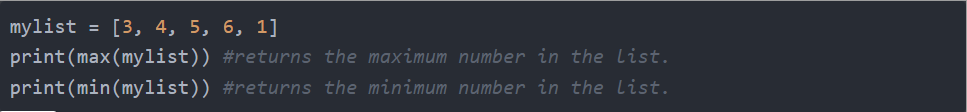
\includegraphics[width=1.0\textwidth]{list-maxmin}
	\caption{Calculate the maximum and minimum of a List}
	\label{fig:list-maxmin}
\end{figure}

\subsection{sum()}
The sum function returns the sum of all the elements in the list.
\begin{figure}[h]
	\centering
	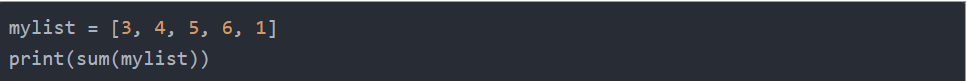
\includegraphics[width=1.0\textwidth]{list-sum}
	\caption{Calculate the sum of a List}
	\label{fig:list-list-sum}
\end{figure}

Output: 19

\subsection{zip()}
Takes iterable containers and returns a single iterator object, having mapped
values from all the containers.

\begin{figure}[h]
	\centering
	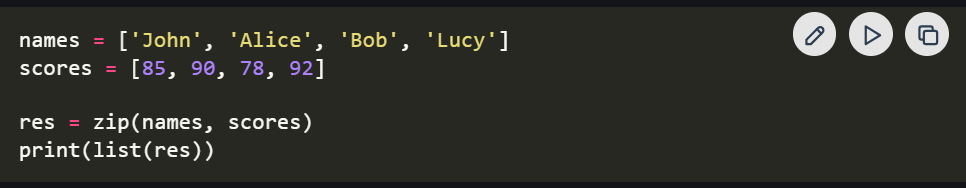
\includegraphics[width=1.0\textwidth]{list-zip}
	\caption{Example of using zip() function}
	\label{fig:list-zip}
\end{figure}
Output: [('John', 85), ('Alice', 90), ('Bob', 78), ('Lucy', 92)]

\subsection{reversed()}
Returns a reversed iterator object.
\newpage
\begin{figure}[h]
	\centering
	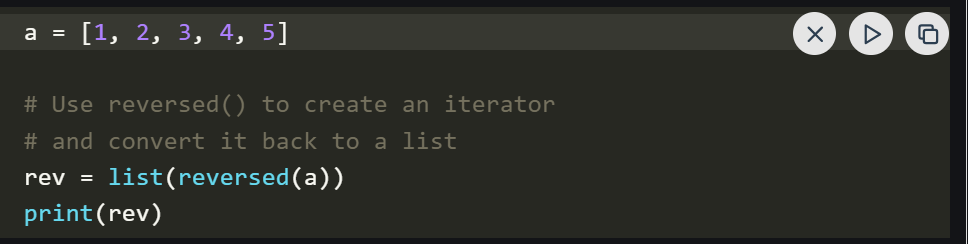
\includegraphics[width=1.0\textwidth]{list-reversed}
	\caption{Example of using reversed() function}
	\label{fig:list-reversed}
\end{figure}
Output: [5, 4, 3, 2, 1]

\subsection{sorted()}
Returns an arranged list. \\
Syntax: sorted(iterable, key=key, reverse=reverse)
\begin{itemize}
	\item iterable - required. The list to sort.
	\item key - optional. A Function to execute to decide the order. Default is None
	\item reverse - optional. A Boolean. False will sort ascending, True will sort descending. Default is False
\end{itemize}

\subsection{enumerate()}
Adds a counter to an iterable and returns it as an enumerate object
(iterator with index and the value) \\
Syntax: enumerate(iterable, start=0)  \\
\begin{itemize}
	\item Iterable: any object that supports iteration
	\item Start: the index value from which the counter is to be started, by default it is 0
\end{itemize}

